\documentclass[12pt,a4paper]{article}
\usepackage{natbib}
\usepackage{graphicx}
\usepackage{float}
\usepackage{multirow}
\usepackage{subfig}
\usepackage{alphalph}
\renewcommand\thesubfigure{\alphalph{\value{subfigure}}}

\begin{document}
\title{Pulsar detection - Machine learning and pattern recognition exam}
\author{Alberto Baroso - s296520}
\date{2022-07-13}
\maketitle
\clearpage

\begin{abstract}
    The Pulsar dataset \cite{stw656} is a collection of 17.898 pulsar candidates of which 1.639 are real pulsars and 16,259 are spurious examples caused by RFI/noise.
    A pulsar is a neutron star that emits beams of electromagnetic radiation.
    As pulsars rotate, their emission beam sweeps across the sky, a periodically repeated pattern of broadband radio emission can be detected as this beam crosses our line of sight.
    Thus pulsar search involves looking for periodic radio signals with large radio telescopes.
    The goal of this project is to use machine learning techniques to solve the binary classification problem of detecting pulsars from the Pulsar dataset.
\end{abstract}
\clearpage

\tableofcontents
\clearpage

\section{Problem analysis}

\subsection{Features}

Pulsar candidates are described by a class label and 8 continuous features extracted from radio signals collected by radio telescopes. \vspace{0.2cm}

The first four are simple statistics obtained from the integrated pulse profile (folded profile).
This is an array of continuous features that describe a longitude-resolved version of the signal that has been averaged in both time and frequency (see \cite{Lyon2016} for more details).
The remaining four features are similarly obtained from the DM-SNR curve (again see \cite{Lyon2016} for more details).
\vspace{0.2cm}
The features are listed below:

\begin{enumerate}
    \item Mean of the integrated profile.
    \item  Standard deviation of the integrated profile.
    \item Excess kurtosis of the integrated profile.
    \item Skewness of the integrated profile.
    \item Mean of the DM-SNR curve.
    \item Standard deviation of the DM-SNR curve.
    \item Excess kurtosis of the DM-SNR curve.
    \item Skewness of the DM-SNR curve.
    \item Class
\end{enumerate}

The class labels used are 0 (non pulsar) and 1 (pulsar).

\subsection{Feature distributions and ranges}

\begin{figure}[H]
    \begin{center}
        \begin{tabular}{cc}
            \subfloat[]{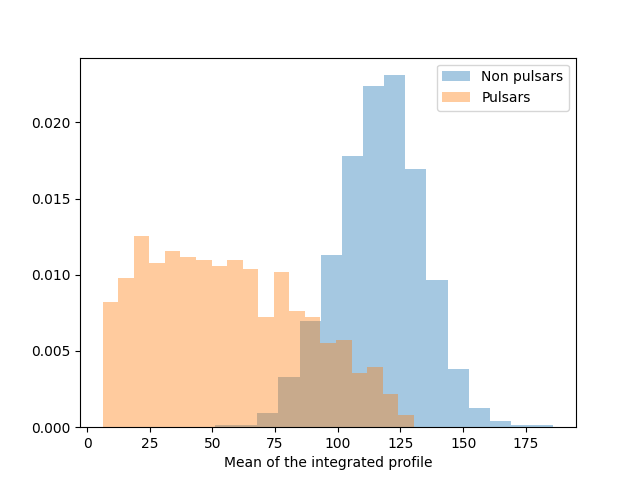
\includegraphics[width = 183pt, height = 120pt]{img/unprocessed_feature_distributions/mean_of_ip.png}}                &
            \subfloat[]{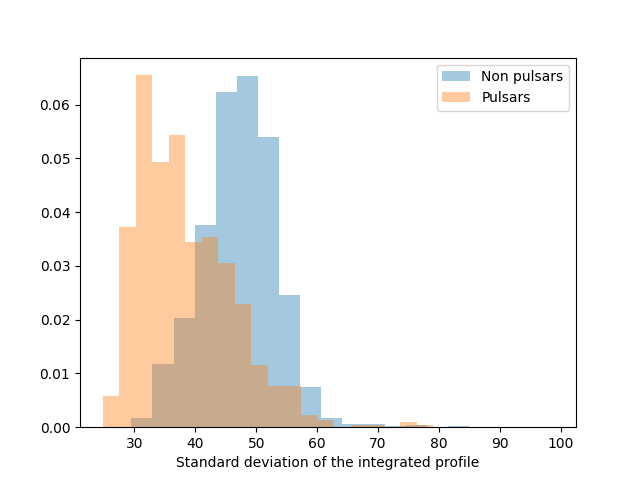
\includegraphics[width = 183pt, height = 120pt]{img/unprocessed_feature_distributions/stdev_of_ip.png}}                 \\
            \subfloat[]{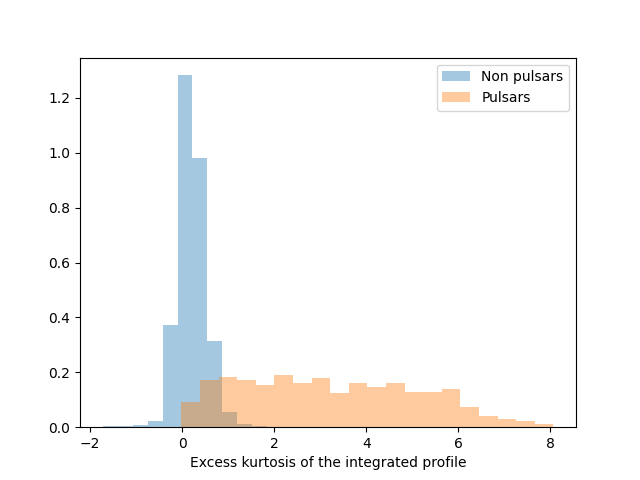
\includegraphics[width = 183pt, height = 120pt]{img/unprocessed_feature_distributions/excess_kurtosis_of_ip.png}}     &
            \subfloat[]{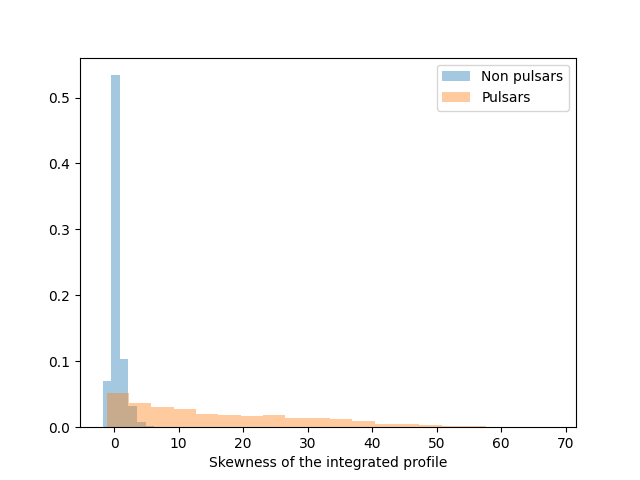
\includegraphics[width = 183pt, height = 120pt]{img/unprocessed_feature_distributions/skewness_of_ip.png}}              \\
            \subfloat[]{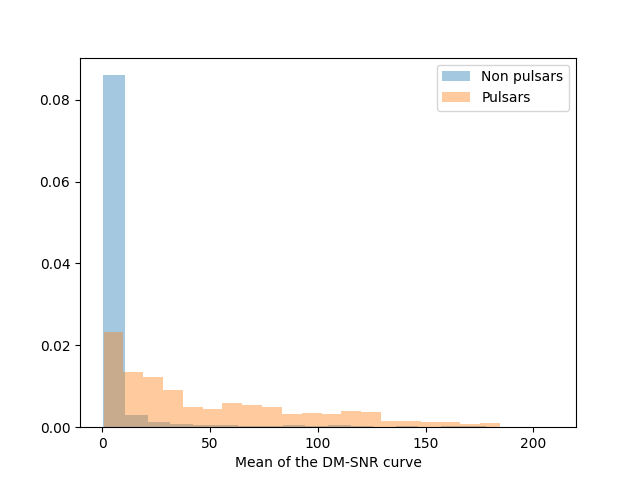
\includegraphics[width = 183pt, height = 120pt]{img/unprocessed_feature_distributions/mean_of_dm-snr.png}}            &
            \subfloat[]{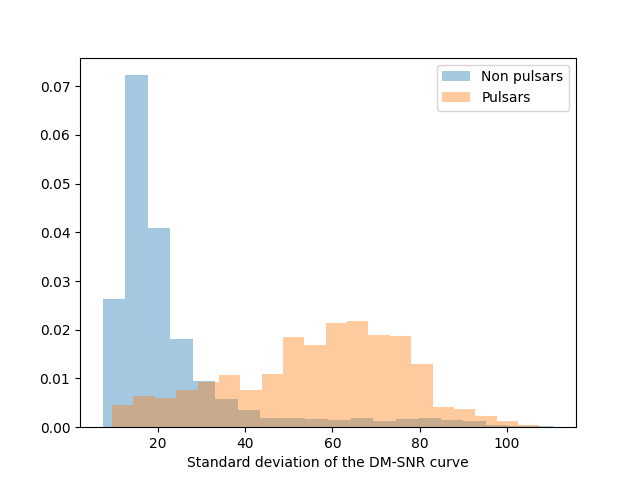
\includegraphics[width = 183pt, height = 120pt]{img/unprocessed_feature_distributions/stdev_of_dm-snr.png}}             \\
            \subfloat[]{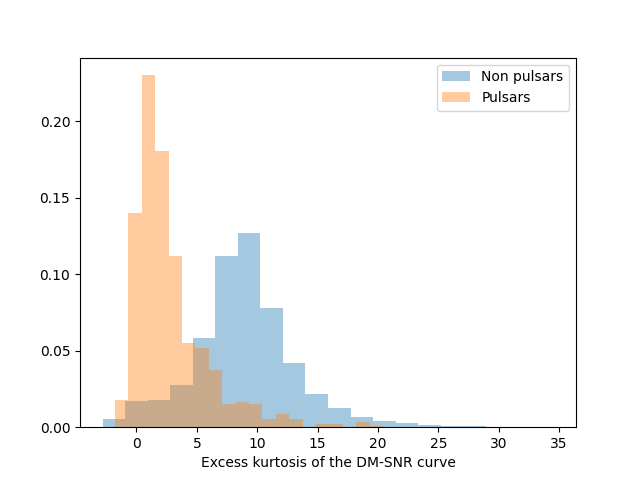
\includegraphics[width = 183pt, height = 120pt]{img/unprocessed_feature_distributions/excess_kurtosis_of_dm-snr.png}} &
            \subfloat[]{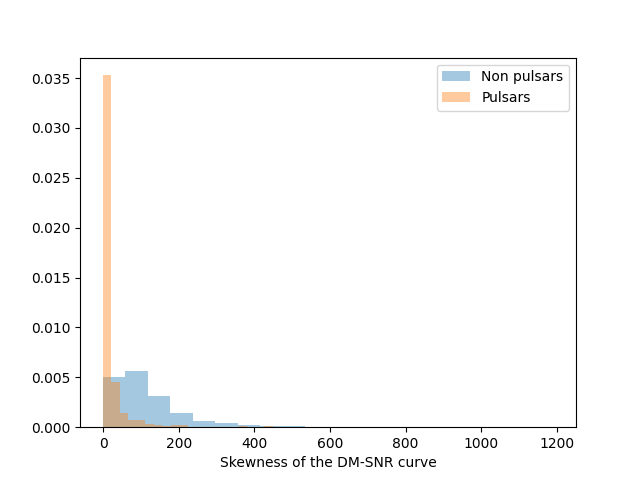
\includegraphics[width = 183pt, height = 120pt]{img/unprocessed_feature_distributions/skewness_of_dm-snr.png}}          \\
        \end{tabular}
    \end{center}
\end{figure}

\begin{minipage}{\linewidth}
    \begin{tabular}{ |c|p{220pt}|p{34pt}|p{30pt}|p{36pt}|  }\hline

           & Feature                                      & Mean   & Min   & Max     \\
        \hline
        a. & Mean of the integrated profile               & 110.86 & 6.18  & 186.02  \\
        \hline
        b. & Standard deviation of the integrated profile & 46.47  & 24.77 & 98.78   \\
        \hline
        c. & Excess kurtosis of the integrated profile    & 0.49   & -1.73 & 8.07    \\
        \hline
        d. & Skewness of the integrated profile           & 1.84   & -1.79 & 68.10   \\
        \hline
        e. & Mean of the DM-SNR curve                     & 12.67  & 0.21  & 209.30  \\
        \hline
        f. & Standard deviation of the DM-SNR curve       & 26.25  & 7.37  & 110.64  \\
        \hline
        g. & Excess kurtosis of the DM-SNR curve          & 8.33   & -2.81 & 34.54   \\
        \hline
        h. & Skewness of the DM-SNR curve                 & 105.41 & -1.98 & 1191.00 \\
        \hline
    \end{tabular}
    \captionof{table}{Feature ranges}
\end{minipage}
\vspace{1cm}

An initial analysis of the raw features of the training data shows that:
\begin{itemize}
    \item Features have mainly irregular distributions
    \item Few features, the ones for non pulsars in figures (a), (b) and (g), present distributions similar to Gaussians
    \item Looking at the graph (b) it's possible to deduce that the "Standard Deviation of the integrated profile" could be one of the less informative features as the histograms of the two classes share one of the largest overlapping areas compared to the other graphs. But since it also has a good amount of non overlapping areas it can still provide useful information for classification purposes.
    \item Grphs (c) and (d) show that "Excess of kurtosis of integrated profile" and "Skewness of integrated profile" could be among the best features for sample discrimination, as they have little overlapping areas of the histograms.
    \item Some features, mainly the ones in graphs (b), (d) and (h), are characterized by the presence of significantly large outliers. Similar claims can be made by looking at the ranges of minimum and maximum values for the corresponding features
    \item We can expect classification algorithms to provide less than ideal results due to the presence of outliers.
\end{itemize}

% As a result, we further pre-process the data by "Gaussianizing" the features.

\subsection{Feature pairs}

\begin{figure}[H]
    \begin{center}
        \begin{tabular}{ccc}
            \hspace*{-65pt}
            \subfloat[]{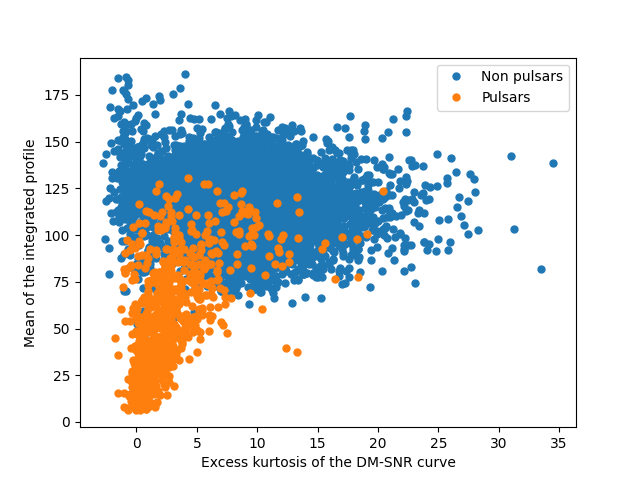
\includegraphics[width = 160pt]{img/unprocessed_feature_pairs/mean_ip-excess_kurtosis_dm-snr.png}} &
            \subfloat[]{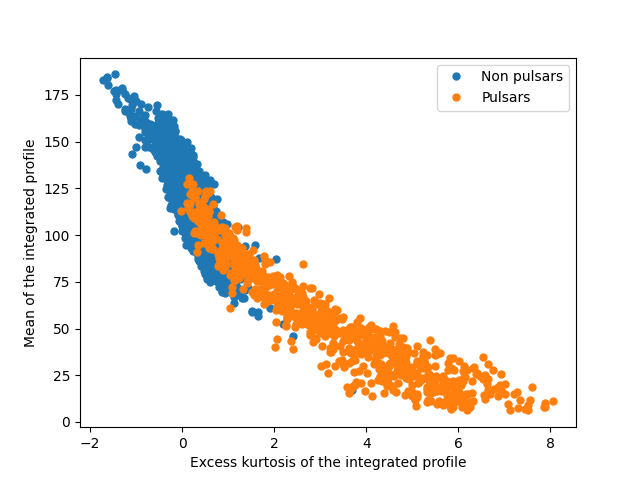
\includegraphics[width = 160pt]{img/unprocessed_feature_pairs/mean_ip-excess_kurtosis_ip.png}}     &
            \subfloat[]{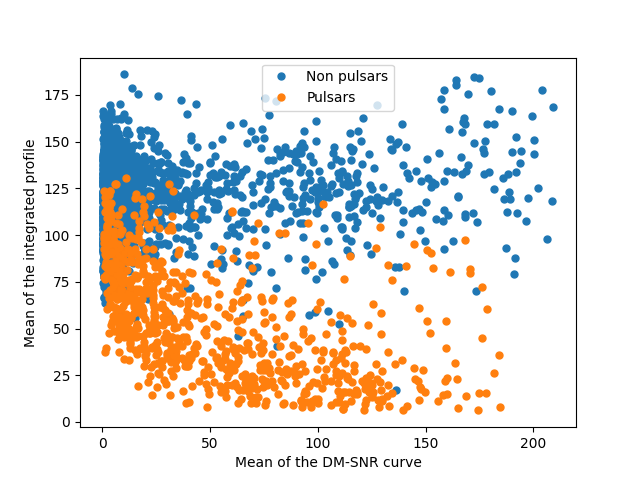
\includegraphics[width = 160pt]{img/unprocessed_feature_pairs/mean_ip-mean_dm-snr.png}}              \\
            \hspace*{-65pt}
            \subfloat[]{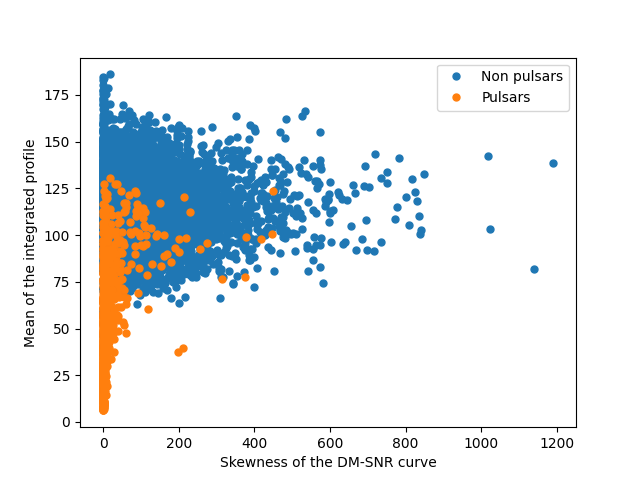
\includegraphics[width = 160pt]{img/unprocessed_feature_pairs/mean_ip-skewness_dm-snr.png}}        &
            \subfloat[]{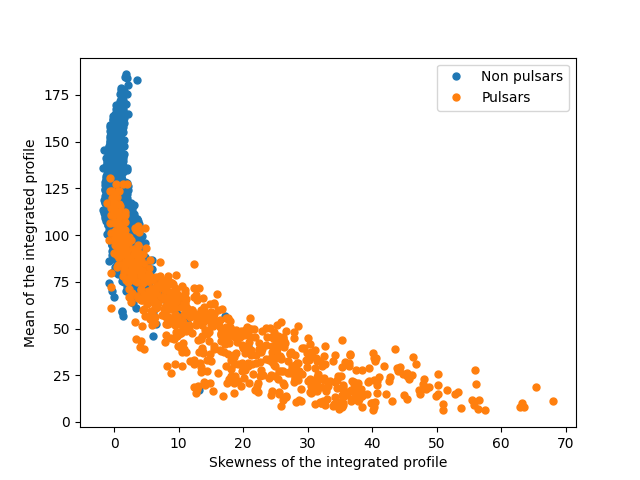
\includegraphics[width = 160pt]{img/unprocessed_feature_pairs/mean_ip-skewness_ip.png}}            &
            \subfloat[]{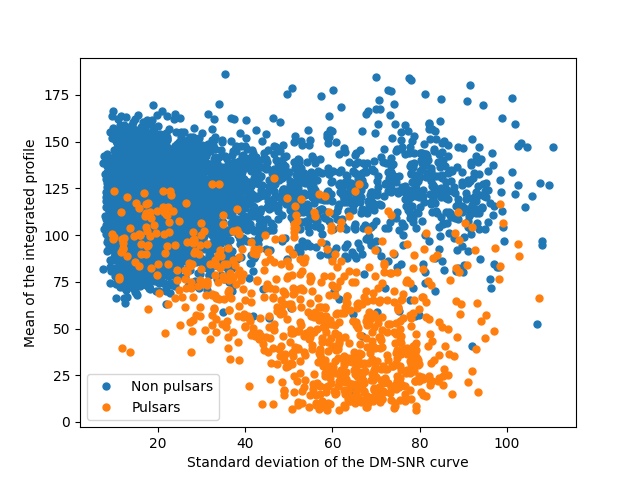
\includegraphics[width = 160pt]{img/unprocessed_feature_pairs/mean_ip-stdev_dm-snr.png}}             \\
            \hspace*{-65pt}
            \subfloat[]{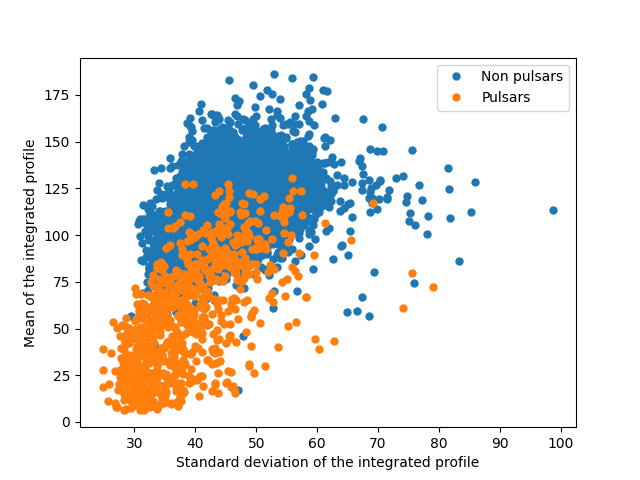
\includegraphics[width = 160pt]{img/unprocessed_feature_pairs/mean_ip-stdev_ip.png}}               &
            \subfloat[]{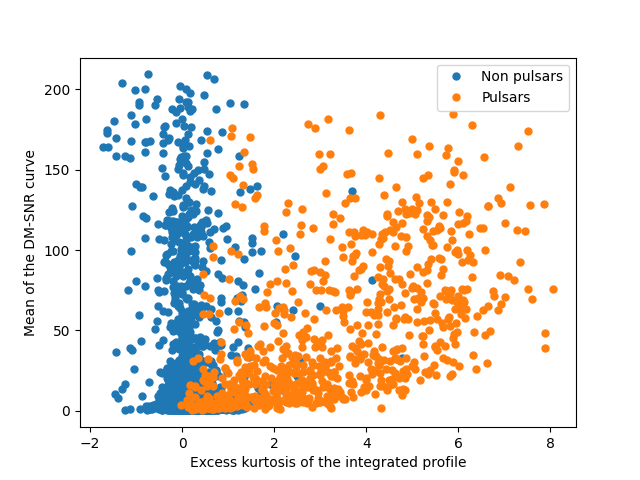
\includegraphics[width = 160pt]{img/unprocessed_feature_pairs/mean_dm-snr-excess_kurtosis_ip.png}} &
            \subfloat[]{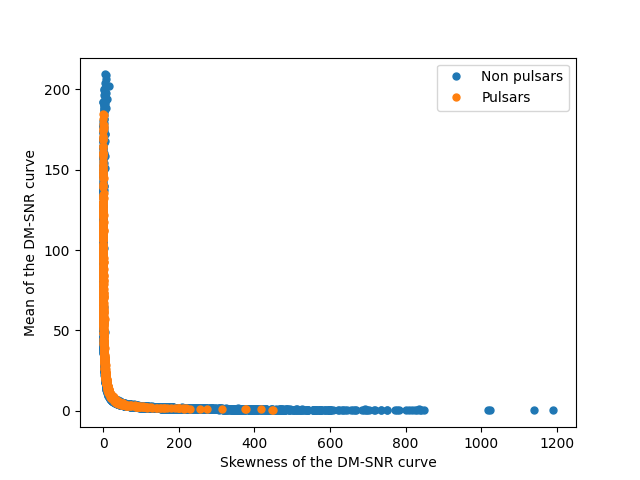
\includegraphics[width = 160pt]{img/unprocessed_feature_pairs/mean_dm-snr-skewness_dm-snr.png}}      \\
            \hspace*{-65pt}
            \subfloat[]{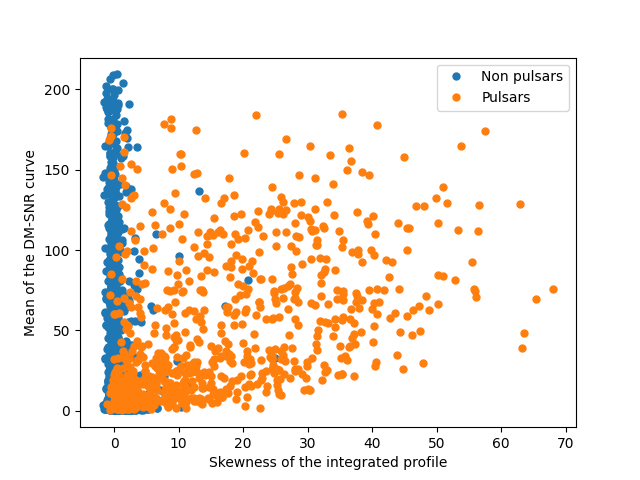
\includegraphics[width = 160pt]{img/unprocessed_feature_pairs/mean_dm-snr-skewness_ip.png}}        &
            \subfloat[]{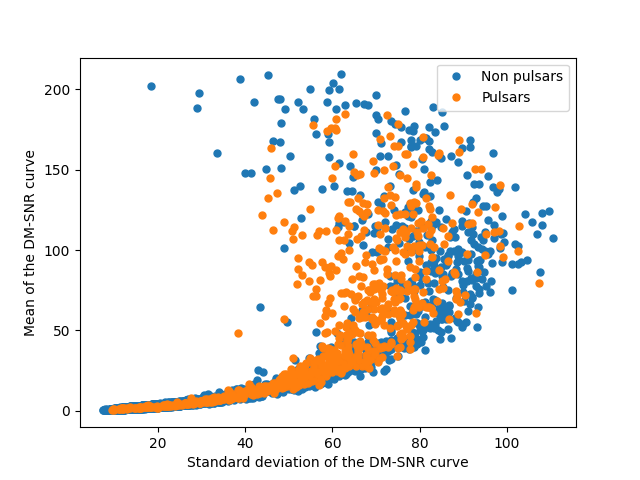
\includegraphics[width = 160pt]{img/unprocessed_feature_pairs/mean_dm-snr-stdev_dm-snr.png}}       &
            \subfloat[]{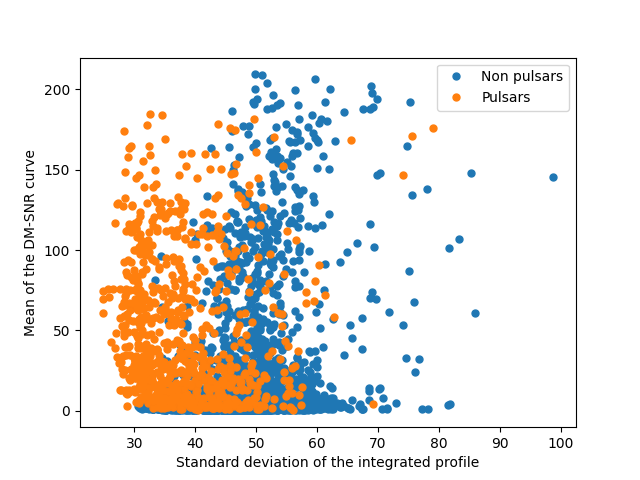
\includegraphics[width = 160pt]{img/unprocessed_feature_pairs/mean_dm-snr-stdev_ip.png}}             \\
        \end{tabular}
    \end{center}
\end{figure}
\begin{figure}[H]
    \begin{center}
        \begin{tabular}{ccc}
            \hspace*{-65pt}
            \subfloat[]{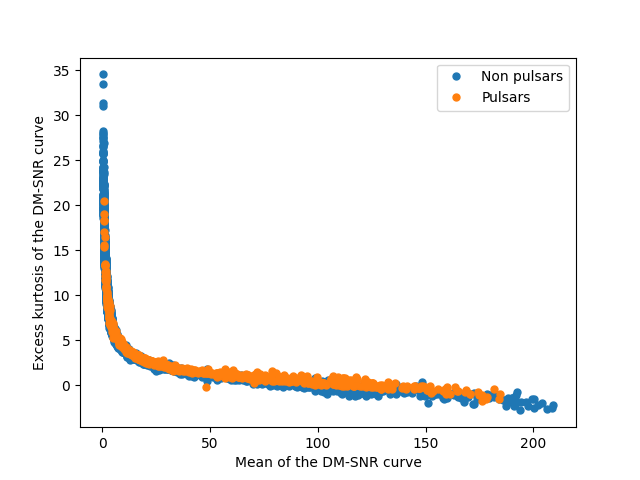
\includegraphics[width = 160pt]{img/unprocessed_feature_pairs/excess_kurtosis_dm-snr-mean_dm-snr.png}}            &
            \subfloat[]{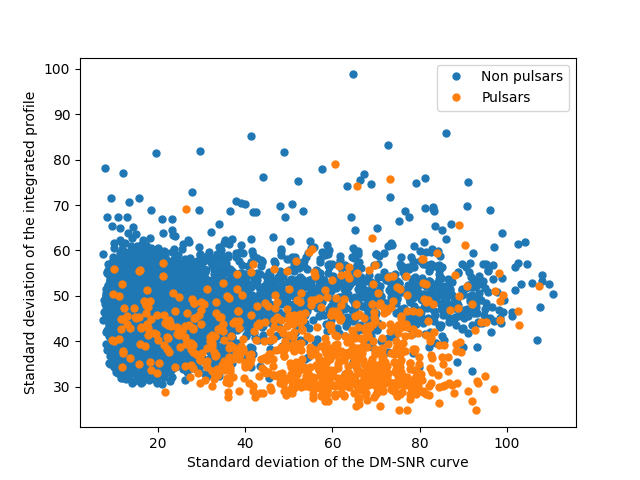
\includegraphics[width = 160pt]{img/unprocessed_feature_pairs/stdev_ip-stdev_dm-snr.png}}                     &
            \subfloat[]{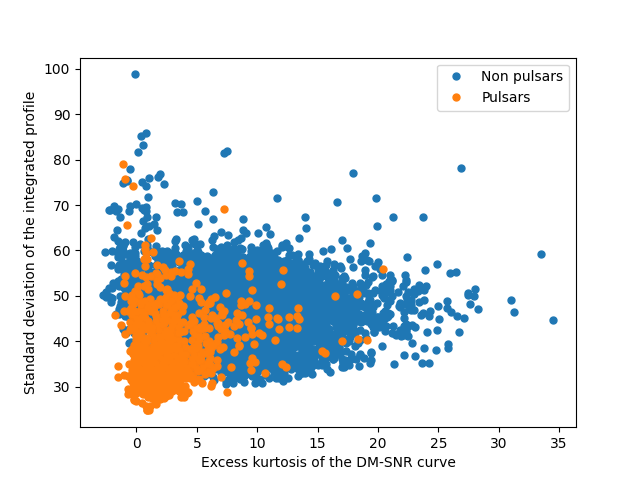
\includegraphics[width = 160pt]{img/unprocessed_feature_pairs/stdev_ip-excess_kurtosis_dm-snr.png}}             \\
            \hspace*{-65pt}
            \subfloat[]{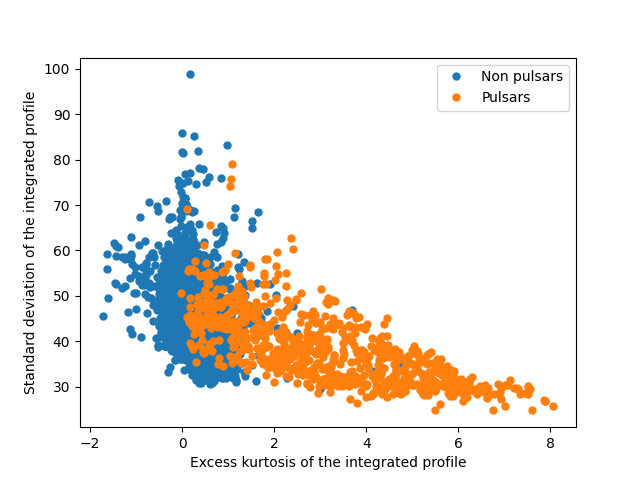
\includegraphics[width = 160pt]{img/unprocessed_feature_pairs/stdev_ip-excess_kurtosis_ip.png}}               &
            \subfloat[]{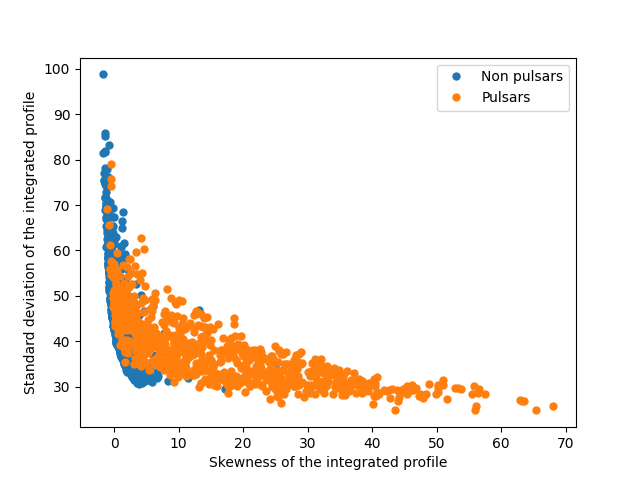
\includegraphics[width = 160pt]{img/unprocessed_feature_pairs/stdev_ip-skewness_ip.png}}                      &
            \subfloat[]{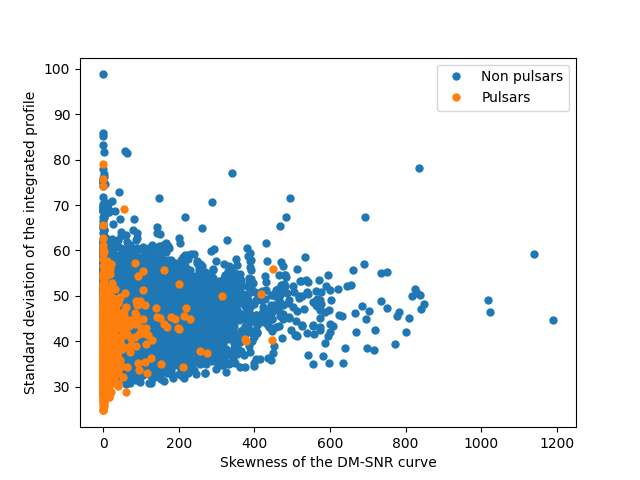
\includegraphics[width = 160pt]{img/unprocessed_feature_pairs/stdev_ip-skewness_dm-snr.png}}                    \\
            \hspace*{-65pt}
            \subfloat[]{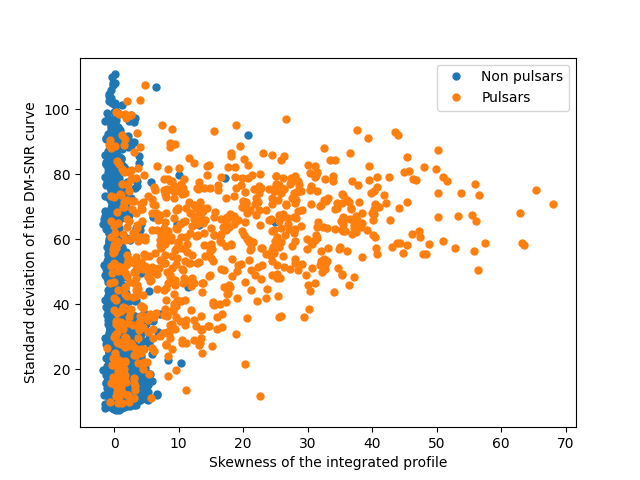
\includegraphics[width = 160pt]{img/unprocessed_feature_pairs/stdev_dm-snr-skewness_ip.png}}                  &
            \subfloat[]{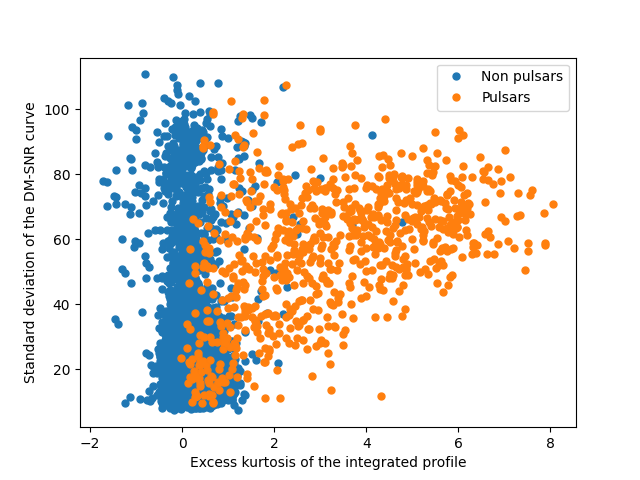
\includegraphics[width = 160pt]{img/unprocessed_feature_pairs/stdev_dm-snr-excess_kurtosis_ip.png}}           &
            \subfloat[]{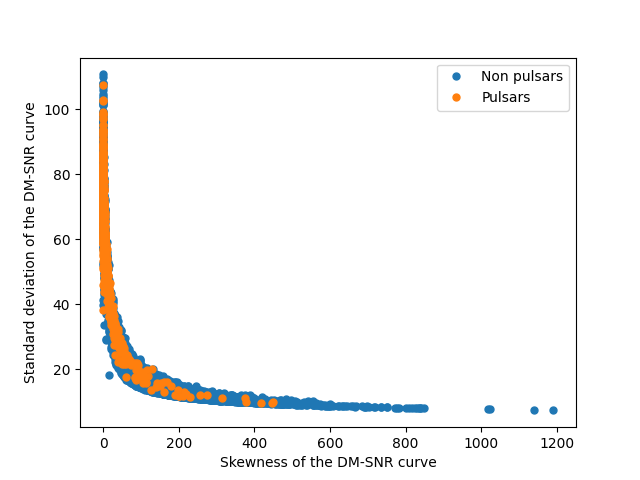
\includegraphics[width = 160pt]{img/unprocessed_feature_pairs/stdev_dm-snr-skewness_dm-snr.png}}                \\
            \hspace*{-65pt}
            \subfloat[]{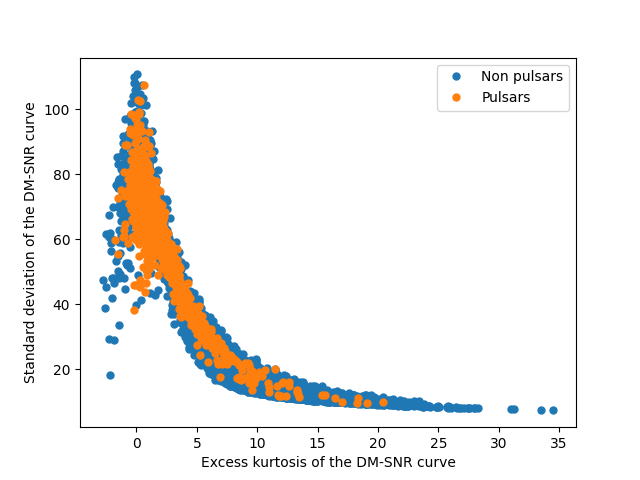
\includegraphics[width = 160pt]{img/unprocessed_feature_pairs/stdev_dm-snr-excess_kurtosis_dm-snr.png}}       &
            \subfloat[]{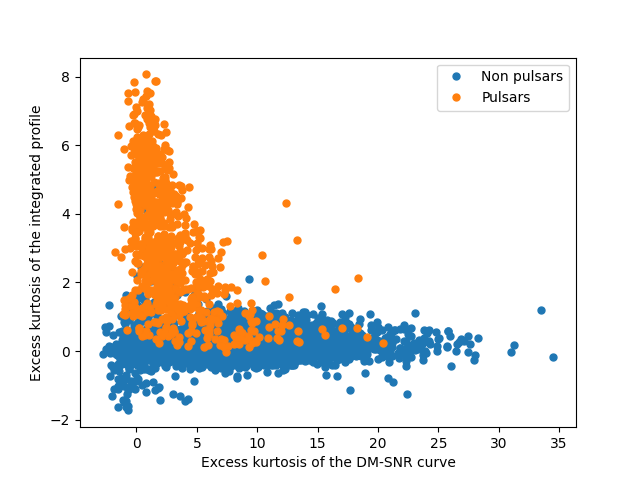
\includegraphics[width = 160pt]{img/unprocessed_feature_pairs/excess_kurtosis_ip-excess_kurtosis_dm-snr.png}} &
            \subfloat[]{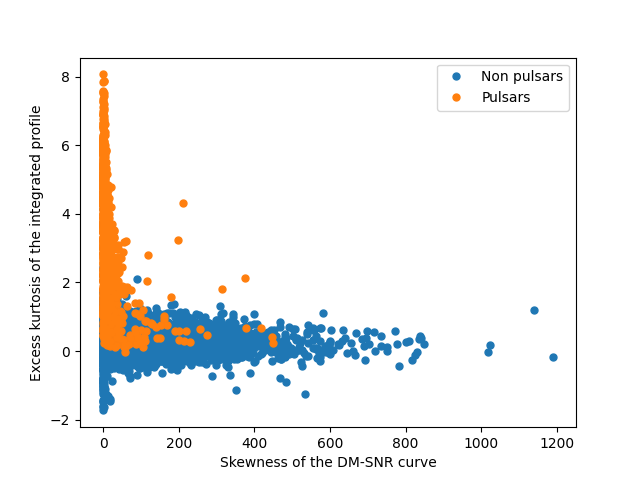
\includegraphics[width = 160pt]{img/unprocessed_feature_pairs/excess_kurtosis_ip-skewness_dm-snr.png}}          \\
        \end{tabular}
    \end{center}
\end{figure}

\begin{figure}
    \begin{center}
        \hspace*{-65pt}
        \begin{tabular}{ccc}
            \subfloat[]{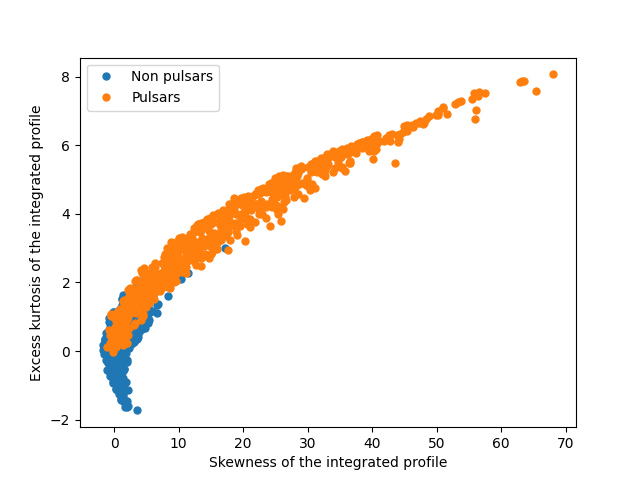
\includegraphics[width = 160pt]{img/unprocessed_feature_pairs/excess_kurtosis_ip-skewness_ip.png}} &
            \subfloat[]{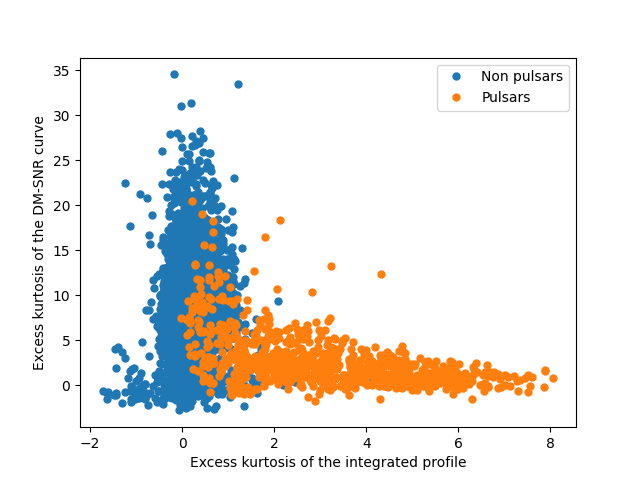
\includegraphics[width = 160pt]{img/unprocessed_feature_pairs/excess_kurtosis_dm-snr-excess_kurtosis_ip.png}} &
            \subfloat[]{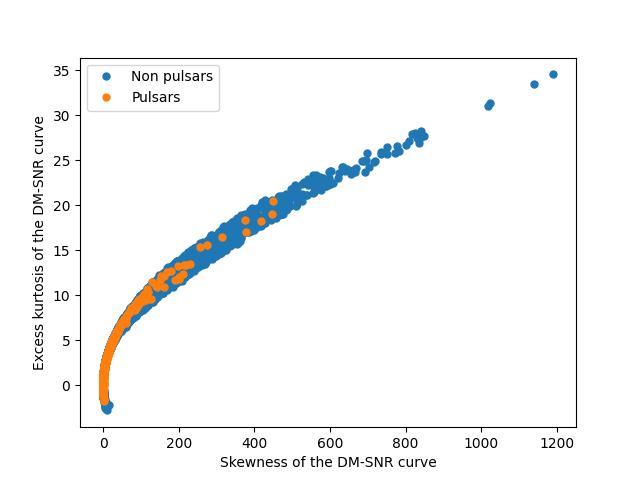
\includegraphics[width = 160pt]{img/unprocessed_feature_pairs/excess_kurtosis_dm-snr-skewness_dm-snr.png}} \\
            \subfloat[]{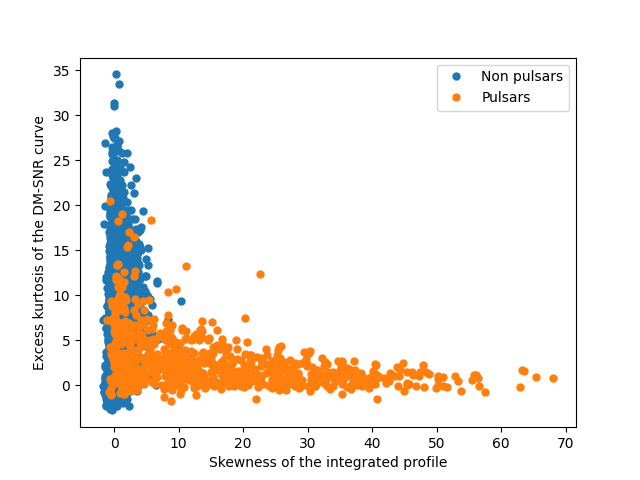
\includegraphics[width = 160pt]{img/unprocessed_feature_pairs/excess_kurtosis_dm-snr-skewness_ip.png}} &
            \subfloat[]{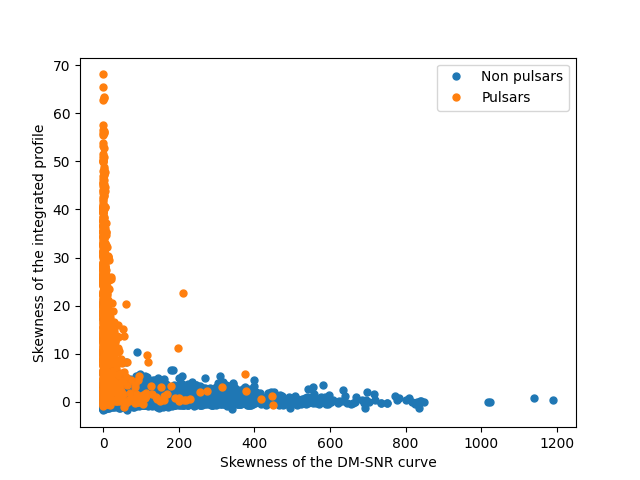
\includegraphics[width = 160pt]{img/unprocessed_feature_pairs/skewness_ip-skewness_dm-snr.png}}  \\
        \end{tabular}
    \end{center}
\end{figure}

% 
% Classes are highly imbalanced.
% 

Observing the feature pairs it's possible to note that there isn't one that allows to find a clear separation of the two classes. 
\vspace*{0.5cm}
The combination of features represented in graphs (n), (p), (ab), (af) and (ah) get close to identify regions of space where samples are well separated.
\vspace*{0.5cm}\\
The least useful pairs of features are represented in graphs (q), (s), (u) and (ac), where samples are almost entirely overlapping.

% TODO: gaussianize features
% TODO: feature correlation: compute pearson correlation heatmap

\clearpage
\bibliographystyle{unsrt}
\bibliography{citations}

\end{document}